\section{Implementation}

Under the NGS regime, candidate solutions will consist of two components:
\begin{enumerate*}[label=(\arabic*)]
\item an initial architecture $A$, and
\item a vector $v$ of network pruning parameters.
\end{enumerate*}
These components will be encoded and recombined separately using standard neuroevolution and genetic algorithm techniques, respectively.
To evaluate a candidate solution, the connection weights of the initial architecture $A$ will be trained for a fixed number of iterations.
Then, a pruning decision will be made for each network node by comparing a cutoff value (defined by $v$) to a quadratic weighting (also defined by $v$) of the following metrics:
\begin{enumerate*}[label=(\alph*)]
\item node activation,
\item correlation of node activation with activation of afferent nodes,
\item correlation of node activation with loss, and
\item backpropagation gradient through the node.
\end{enumerate*}
Following pruning, training will resume for a fixed number of iterations. Candidate solution fitness will be assessed as the validation set performance of the final trained network.
Figure 1 compares NGS with existing methods.

\noindent
\begin{minipage}{0.8\textwidth}
 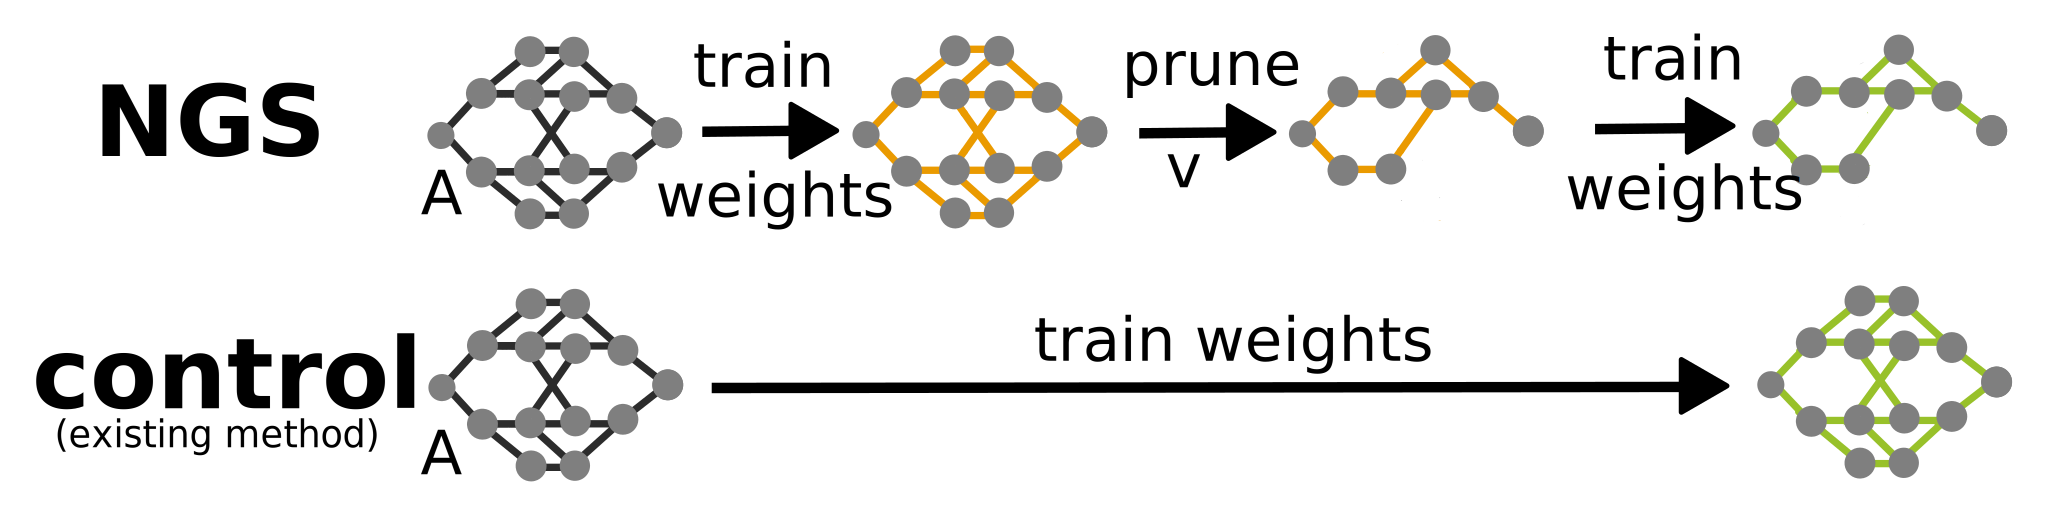
\includegraphics[width=\textwidth]{img/complete}
\end{minipage}%
\begin{minipage}{0.2\textwidth}
  {\setstretch{0.7}
  \begin{footnotesize}
    \textit{
   Figure 1: A schematic comparison of a candidate NGS solution (top) with a candidate solution under existing methods (bottom).
   }
  \end{footnotesize}
  \par}
\end{minipage}

\section{Research Plan}

First, I will conduct \textbf{exploratory experiments to assess the capacity of NGS to promote parsimony, irregular refinement, evolvability, and adaptive plasticity} at the Michigan State University High Performance Computing Center.
For these experiments, I will use the HyperNEAT encoding, a standard indirect encoding for artificial neuroevolution \cite{clune2011performance}.
I will evolve ANN architectures for a variant of the bit mirroring problem, which is designed to enable experimental manipulation of symmetry in the problem domain.
The capacity of NGS to enable irregular refinement will be assessed by comparing NGS-HyperNEAT and control (i.e. HyperNEAT) performance across a spectrum of problem regularities.
Greater relative performance of NGS-HyperNEAT at low problem regularity would confirm that NGS enables irregular refinement.
I will assess the impact of NGS on evolvability by comparing between NGS and control treatments the phenotypic novelty and viability of mutant offspring of evolved architectures and the rate at which evolving populations adapt to altered evolutionary objectives \cite{tarapore2015evolvability}.
I will test the impact of NGS on adaptive plasticity by comparing between NGS and control treatments the ability of architectures evolved to handle one set of bit mirroring symmetries to perform on a bit mirroring problem with different symmetries.
Finally, I will compare the impact of parsimony selection pressure on performance and network size for NGS and control treatments.
I expect NGS to boost parsimony, irregular refinement, evolvability, and adaptive plasticity.

Next, I will \textbf{assess the performance of NGS-enabled architecture evolution on benchmark deep learning datasets}.
I will leverage the results of my exploratory experiments to \textbf{seek collaborators in industry} for these benchmarking experiments through connections between my research group and Sentient.
These experiments will employ the CoDeepNEAT encoding \cite{miikkulainen2017evolving}, an indirect encoding developed specially to evolve deep learning architectures.
I will benchmark NGS-CoDeepNEAT against existing results for CoDeepNEAT on datasets for computer vision (CIFAR-10/100) and language modeling (PTB).
I expect performance to meet or exceed state-of-the-art.
